The damage function maps hazard intensity to a damage ratio $\DF \in [0,1]$, representing the repair cost as a fraction of replacement value. We adopt the generalised logistic (Richards) function as our parametric form:

\begin{equation}
    Y(x) = A + \frac{K - A}{\left( C + Q \exp{[-B(x - a)]} \right)^{\frac{1}{\nu}}}
    \label{eq: logistic function}
\end{equation}
with $A = 0$, $K = 1$, $C = 1$ for damage ratios bounded in $[0,1]$. The remaining parameters have clear physical interpretations: $B$ controls the steepness of the damage curve (how rapidly damage increases with depth); $a$ sets the inflection point (the depth at which damage reaches approximately 50\%); $Q$ affects onset speed (how quickly damage departs from zero); and $\nu$ controls asymmetry (whether damage accelerates faster at low or high depths).

\begin{figure}[ht]
\centering
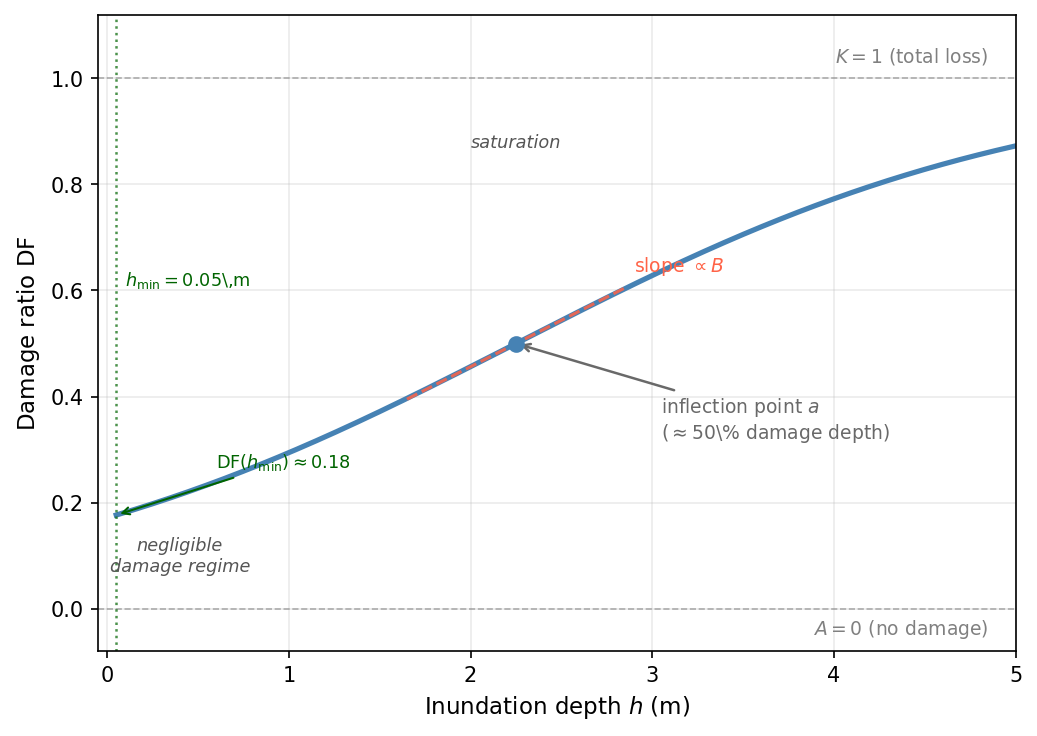
\includegraphics[width=0.75\textwidth]{Content/Images/richards_schematic.png}
\caption{Schematic Richards damage function: the S-shaped curve transitions from negligible damage at low depths through a steep transition (controlled by $B$) centred at inflection point $a$ to saturation near total loss. Note: the Richards function approaches $\DF = 0$ only asymptotically as $h \to -\infty$; at $h = 0$ the function takes a small positive value ($\approx 0.19$ for the calibrated parameters), reflecting the minimum-damage floor below which flooding is not practically relevant. Curves are plotted from $h_{\min} = 0.05$\,m.}
\label{fig: damage function}
\end{figure}

The Richards function has sufficient flexibility to capture the main features of empirical depth-damage relationships --- an initial low-damage regime, a rapid transition, and saturation near total loss --- while remaining parsimonious enough (four free parameters for a single-variable, instantaneous function) to avoid overfitting on noisy insurance claims data.

The calibration output is a parameter set $(a, B, Q, \nu)$ for each combination of hazard type and asset category:
\begin{equation*}
    \text{Category}_i, \text{ Hazard}_j : \quad (a_{ij}, B_{ij}, Q_{ij}, \nu_{ij})
    %\label{eq: calibration result}
\end{equation*}
In this paper, we calibrate for the flood--residential combination using FEMA data (Section~\ref{sec: empirical}) and bridge to commercial assets via the sector adjustment (Section~\ref{ssec: sector}).
